% Enable warnings about problematic code
\RequirePackage[l2tabu, orthodox]{nag}

\documentclass{WeSTassignment}

% The lecture title, e.g. "Web Information Retrieval".
\lecture{Introduction to Web Science}
% The names of the lecturer and the instructor(s)
\author{%
  Prof. Dr.~Steffen~Staab\\{\normalsize\mailto{staab@uni-koblenz.de}} \and
  Ren{\'e}~Pickhardt\\{\normalsize\mailto{rpickhardt@uni-koblenz.de}} \and
   Korok~Sengupta\\{\normalsize\mailto{koroksengupta@uni-koblenz.de}}
}
% Assignment number.
\assignmentnumber{1}
% Institute of lecture.
\institute{%
  Institute of Web Science and Technologies\\%
  Department of Computer Science\\%
  University of Koblenz-Landau%
}
% Date until students should submit their solutions.
\datesubmission{November 2, 2016, 10:00 a.m.}
% Date on which the assignments will be discussed in the tutorial.
\datetutorial{November 4th, 2016, 12:00 p.m.}

% Set langauge of text.
\setdefaultlanguage[
  variant = american, % Use American instead of Britsh English.
]{english}

% Specify bib file location.
\addbibresource{bibliography.bib}

% For left aligned centerd boxes
% see http://tex.stackexchange.com/a/25591/75225
\usepackage{varwidth}

% ==============================================================================
% Document

\begin{document}

\maketitle

The main objective of this assignment is for you to use different tools with which you can understand the network that you are connected to or you are connecting to in a better sense.
These tasks are not always specific to \enquote{Introduction to Web Science}.
For all the assignment questions that require you to write a code, make sure to include the code in the answer sheet, along with a separate python file. Where screen shots are required, please add them in the answers directly and not as separate files. \\
\\

% As such, this assignment will not award any points, and you will \emph{not} have
% to submit your solution.
% If you want to know whether your solutions were correct, mail them to
% \mailto{lukas@uni-koblenz.de}.
\\
\\
\\
\\ 
{\Large Group name: echo\par} \\
{\Large Group Member: Hanadi Tamimi, Keya Kashem, Md Jakaria Nawaz\par} \\
% ------------------------------------------------------------------------------

\section{Ethernet Frame (5 Points)}

Ethernet Frame is of the given structure:
\begin{figure}[h]
  \centering
  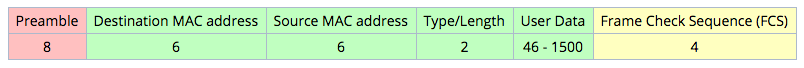
\includegraphics[width=0.9\textwidth]{1.png}
   \caption{Ethernet Frame Structure}
     \label{fig:ethernet}
\end{figure}

Given below is an Ethernet frame without the Preamble and the Frame Check Sequence.\\ 
 
\texttt{00 27 10 21 fa 48 00 13 \hspace{0.5cm} 10 e8 dd 52 08 06 00 01\\ 08 00 06 04 00 01 00 13 \hspace{0.5cm} 10 e8 dd 52 c0 a8 02 01\\ 00 00 00 00 00 00 c0 a8 \hspace{0.5cm} 02 67} \\ \\

\underline{Find}:
\begin{enumerate}
\item Source MAC Address
\item Destination MAC Address
\item What protocol is inside the data payload?
\item Please mention what the last 2 fields hold in the above frame.
\end{enumerate}

%Answer
\underline{Answers:}

\begin{enumerate}
\item 00 13 10 e8 dd 52
\item 00 27 10 21 fa 48
\item The type length has two bytes. If the hex value is less than 06 00 then it indicates the field is used as the size of the payload of the Ethernet frame. But if the hex value is more than 06 00 then the field is used to represent EtherType. Here it is 08 06 > 06 00. So it represents EtherType and 08 06 indicates Address Resolution Protocol (ARP).
\item The last one indicates the amount of data is being transferred. The range is 46-1500 bytes. In this case the data: 00 01 08 00 06 04 00 01 00 13 10 e8 dd 52 c0 a8 02 01 00 00 00 00 00 00 c0 a8 02 67 00 00 00 00 00 00 00 00 00 00 00 00 00 00 00 00 00 00 \\
\\
The field before that indicates either EtherType (if HexValue > 0600) or size of the payload (if HexValue < 0600).

\end{enumerate}

% ------------------------------------------------------------------------------

\section{Cable Issue (5 Points)}

Let us consider we have two cables of 20 meters each. One of them is in a 100MBps network while the other is in a 10MBps network. If you had to transfer data through each of them, how much time it would take for the first bit to arrive in each setting? (For your calculation you can assume that the speed of light takes the same value as in the videos.) Please provide formulas and calculatoins along with your results. 


%Answer
\underline{Answers:}
\begin{enumerate}
\item Cable length 20 m \\ 
Network bandwidth 100MBps = 100 Million bits per second \\ 
Or 1 bit per $(1 /100 Million)$ seconds or 0.00000001 seconds or 10 nanoseconds.\\ 
The speed of light = 299792458 m/s. (Data will pass in this speed as electromagnetic wave) \\
In 1 sec data travel 299792458 m [in 100MBps Cable] \\
So, in .00000001 sec 1 bit will travel $(299792458*0.00000001)m$ = 2.998 m \\
So,  to travel 20 meters it will take ${(20*10)/2.998} nanoseconds$ = 66.71 nanoseconds\\


\item Cable length 20 m \\ 
Network bandwidth 10MBps = 10 Million bits per second \\ 
Or 1 bit per $(1 /10 Million)$ seconds or 0.0000001 seconds or 100 nanoseconds.\\ 
The speed of light = 299792458 m/s. (Data will pass in this speed as electromagnetic wave) \\
In 1 sec data travel 299792458 m [in 100MBps Cable] \\
So, in .0000001 sec 1 bit will travel $(299792458*0.0000001)m$ = 29.9792 m \\
So,  to travel 20 meters it will take ${(20*100)/29.979} nanoseconds$ = 66.71 nanoseconds\\

\end{enumerate}

% ------------------------------------------------------------------------------


\section{Basic Network Tools (10 Points)}

Listed below are some of the commands which you need to "google" to understand what they stand for:
\begin{enumerate}
\item \emph{ipconfig / ifconfig}
\item \emph{ping}
\item \emph{traceroute}
\item \emph{arp}
\item \emph{dig}
\end{enumerate}

Consider a situation in which you need to check if \url{www.wikipedia.org} is reachable or not. Using the knowledge you gained above to \underline{find the following information}:
\begin{enumerate}
\itemsep0em
\item The \emph{\% packet loss} if at all it happened after sending 100 packets. 
\item \emph{Size} of the packet sent to \emph{Wikipedia} server
\item \emph{IP address} of your machine and the \emph{Wikipedia} server
\item \emph{Query Time} for DNS query of the above url.
\item Number of \emph{Hops} in between your machine and the server
\item MAC address of the device that is acting as your network gateway. 
\end{enumerate}

Do this once in the university and once in your home/dormitory network. With your answers, you must paste the screen shots to validate your find.


%Answer
\underline{Answers:}
\begin{enumerate}
\item \\
\underline{Home:} After sending 100 packets of data the percentage of packet loss is 0.(ping -c 100 www.wikipedia.org) \\
\\
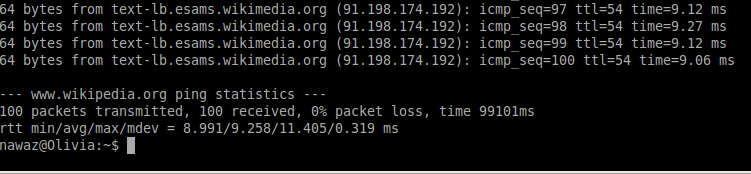
\includegraphics[width=1\textwidth]{images/home-packet-loss(1-1).png}
\\
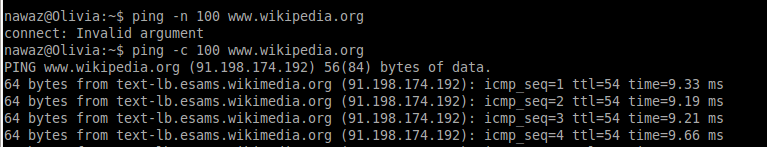
\includegraphics[width=1\textwidth]{images/home-packet-loss(1-2).png}
\\
\underline{University:} After sending 100 packets of data the percentage of packet loss is 0.(ping -n 100 www.wikipedia.org) \\
\\
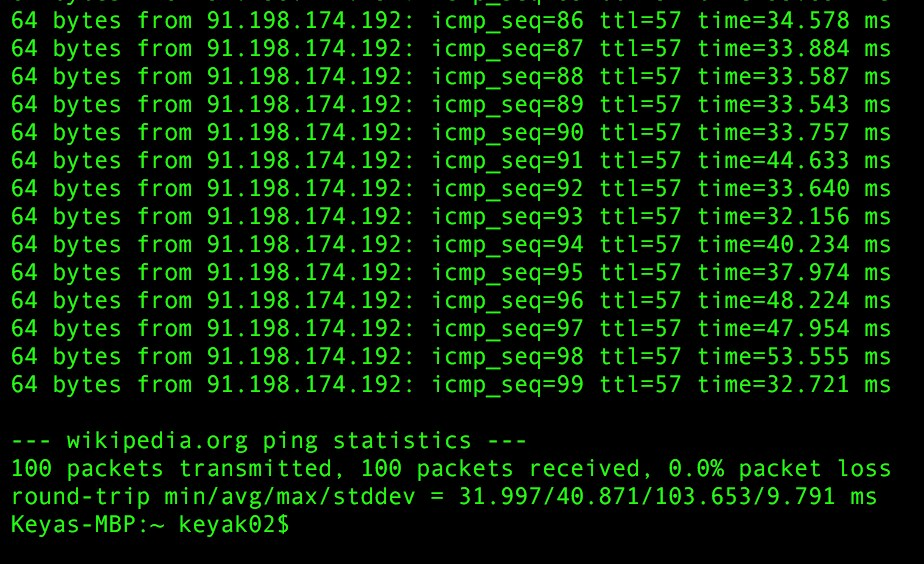
\includegraphics[width=1\textwidth]{images/out-packet-loss(1-0).png}
\\
\item \\
\underline{Home:} Size of the packet sent to wikipedia server is 56 bytes. (ping www.wikipedia.org) \\
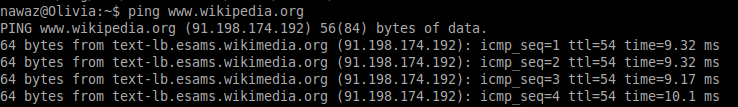
\includegraphics[width=1\textwidth]{images/home-packet-size(2-0).png}
\\
\underline{University:} Size of the packet sent to wikipedia server is 56 bytes. (ping www.wikipedia.org) \\
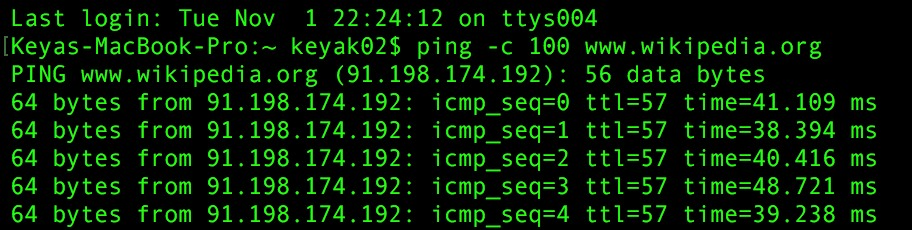
\includegraphics[width=1\textwidth]{images/out-packet-size(2-0).png}
\\
\item \\
\underline{Home:} IP address of machine - 172.16.5.57 . (ifconfig) \\
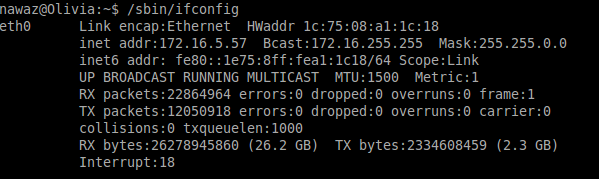
\includegraphics[width=1\textwidth]{images/home-machine-IP(3-1).png}
\\
IP address of wikipedia server 97.198.174.192 . (ping www.wikipedia.org) \\
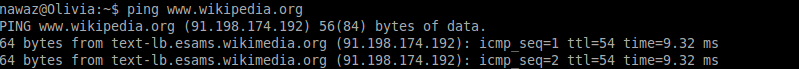
\includegraphics[width=1\textwidth]{images/home-wiki-IP(3-2).png}
\\
\underline{University:} IP address of machine - 192.168.178.51 . (ifconfig) \\
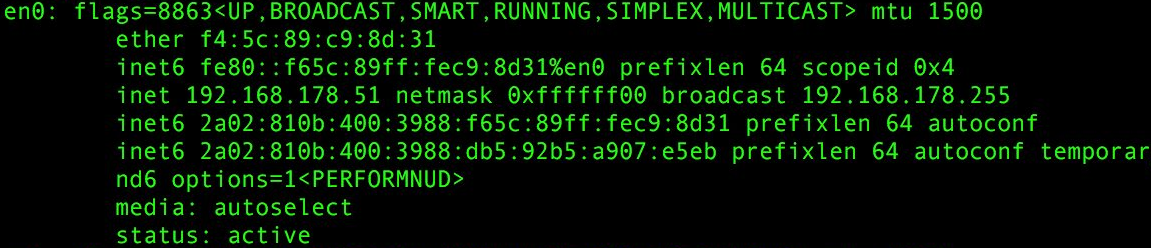
\includegraphics[width=1\textwidth]{images/out-machine-IP(3-1).png}
\\
IP address of wikipedia server 97.198.174.192 . (ping www.wikipedia.org) \\
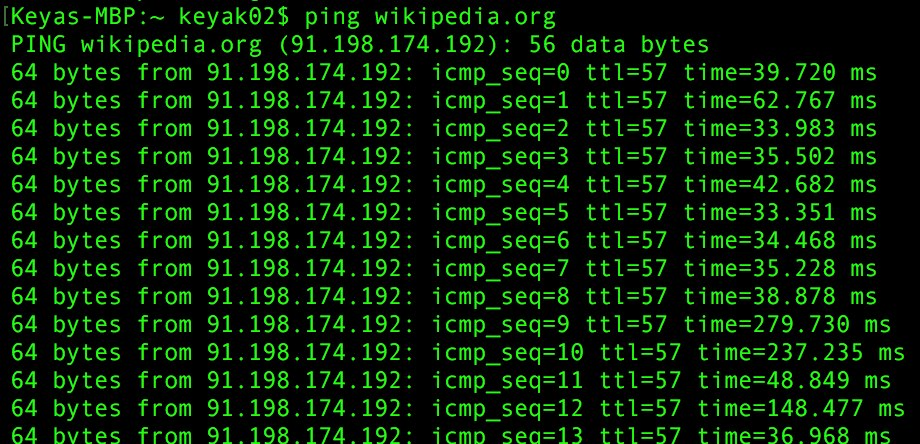
\includegraphics[width=1\textwidth]{images/out-wiki-IP(3-2).png}
\\
\item \\
\underline{Home:} Query time for DNS query of www.wikipedia.org - 13 msec . (dig www.wikipedia.org) \\
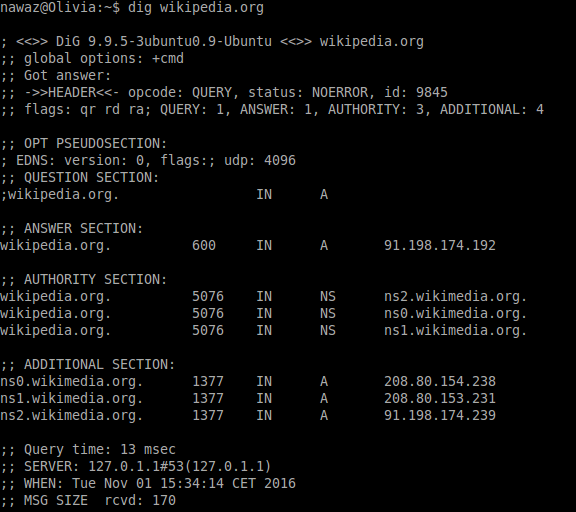
\includegraphics[width=1\textwidth]{images/home-query-time(4-0).png}
\\
\underline{University:} Query time for DNS query of www.wikipedia.org - 41 msec . (dig www.wikipedia.org) \\
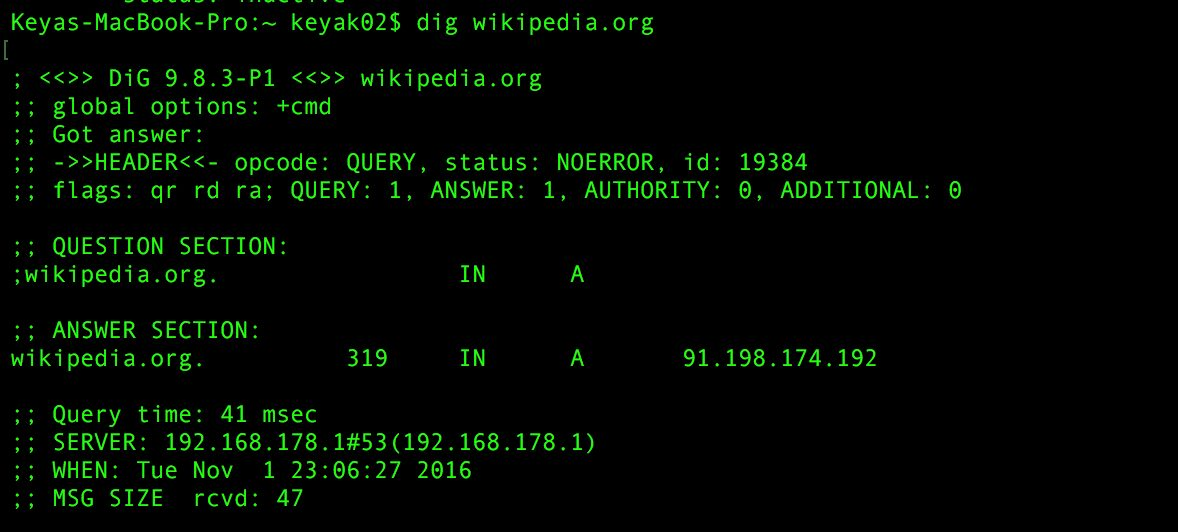
\includegraphics[width=1\textwidth]{images/out-query-time(4-0).png}
\\
\item \\
\underline{Home:} It took 9 hops to reach www.wikipedia.org server. (traceroute www.wikipedia.org) \\
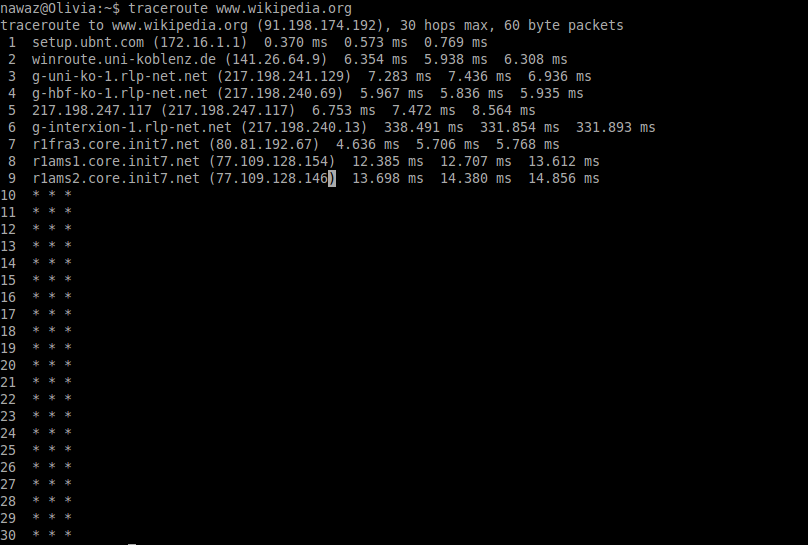
\includegraphics[width=1\textwidth]{images/home-hops(5-0).png}
\\
\underline{University:} It took 6 hops to reach www.wikipedia.org server. (traceroute www.wikipedia.org) \\
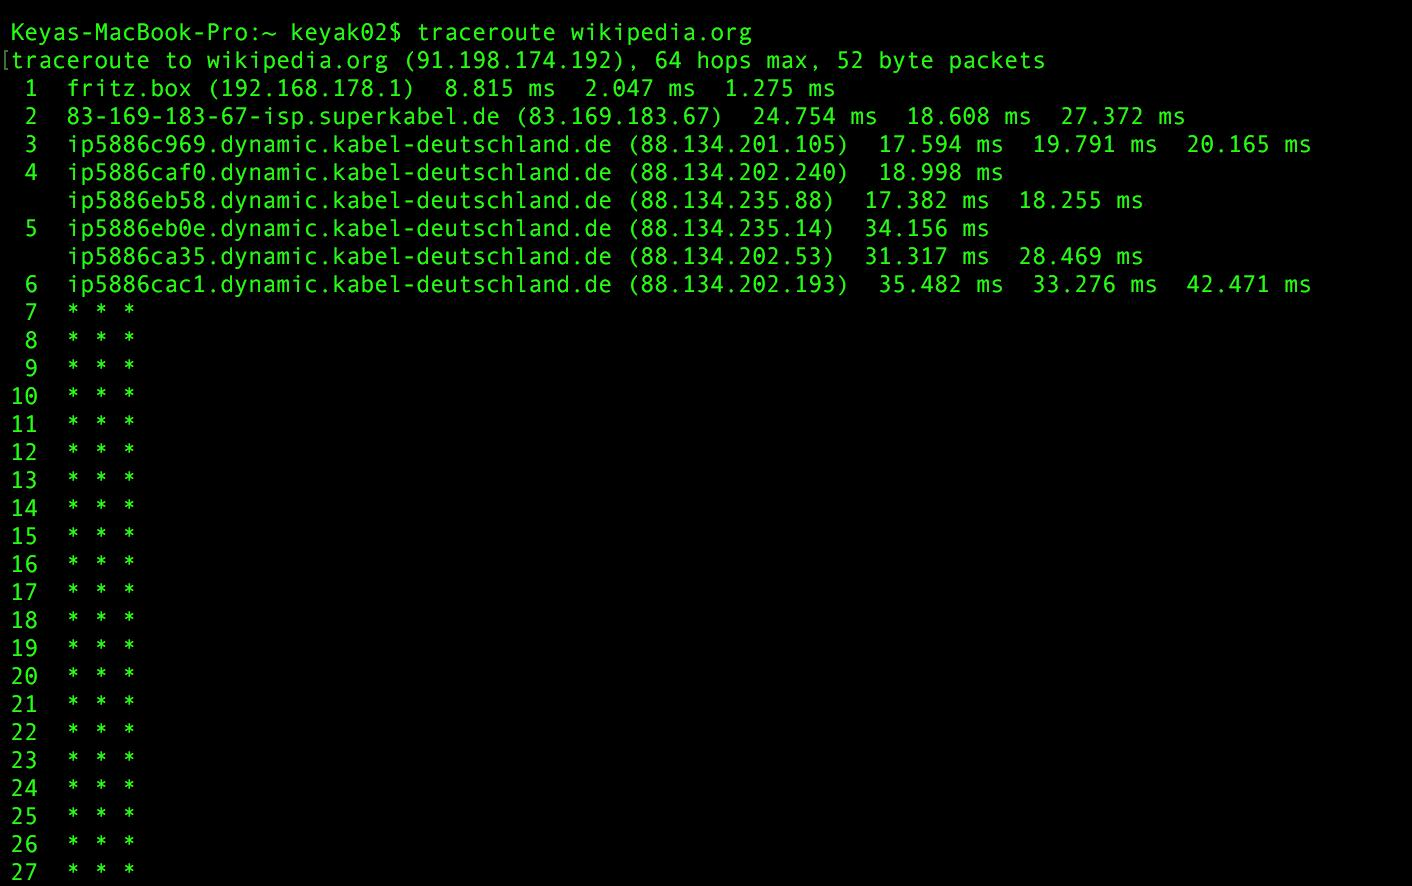
\includegraphics[width=1\textwidth]{images/out-hops(5-0).png}
\\
\item \\
\underline{Home:} MAC address of network gateway 04:18:d6:83:a9:83. (route -n, arp -n) \\
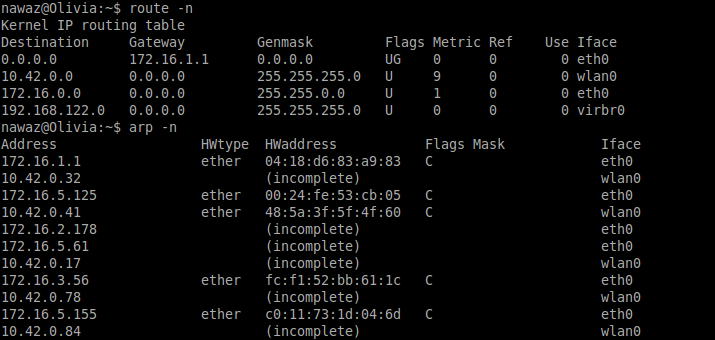
\includegraphics[width=1\textwidth]{images/home-gateway-mac(6-0).png}
\\
\underline{University:} MAC address of network gateway 34:31:c4:7d:65:8a. (netstat -nr, for macintosh device) \\
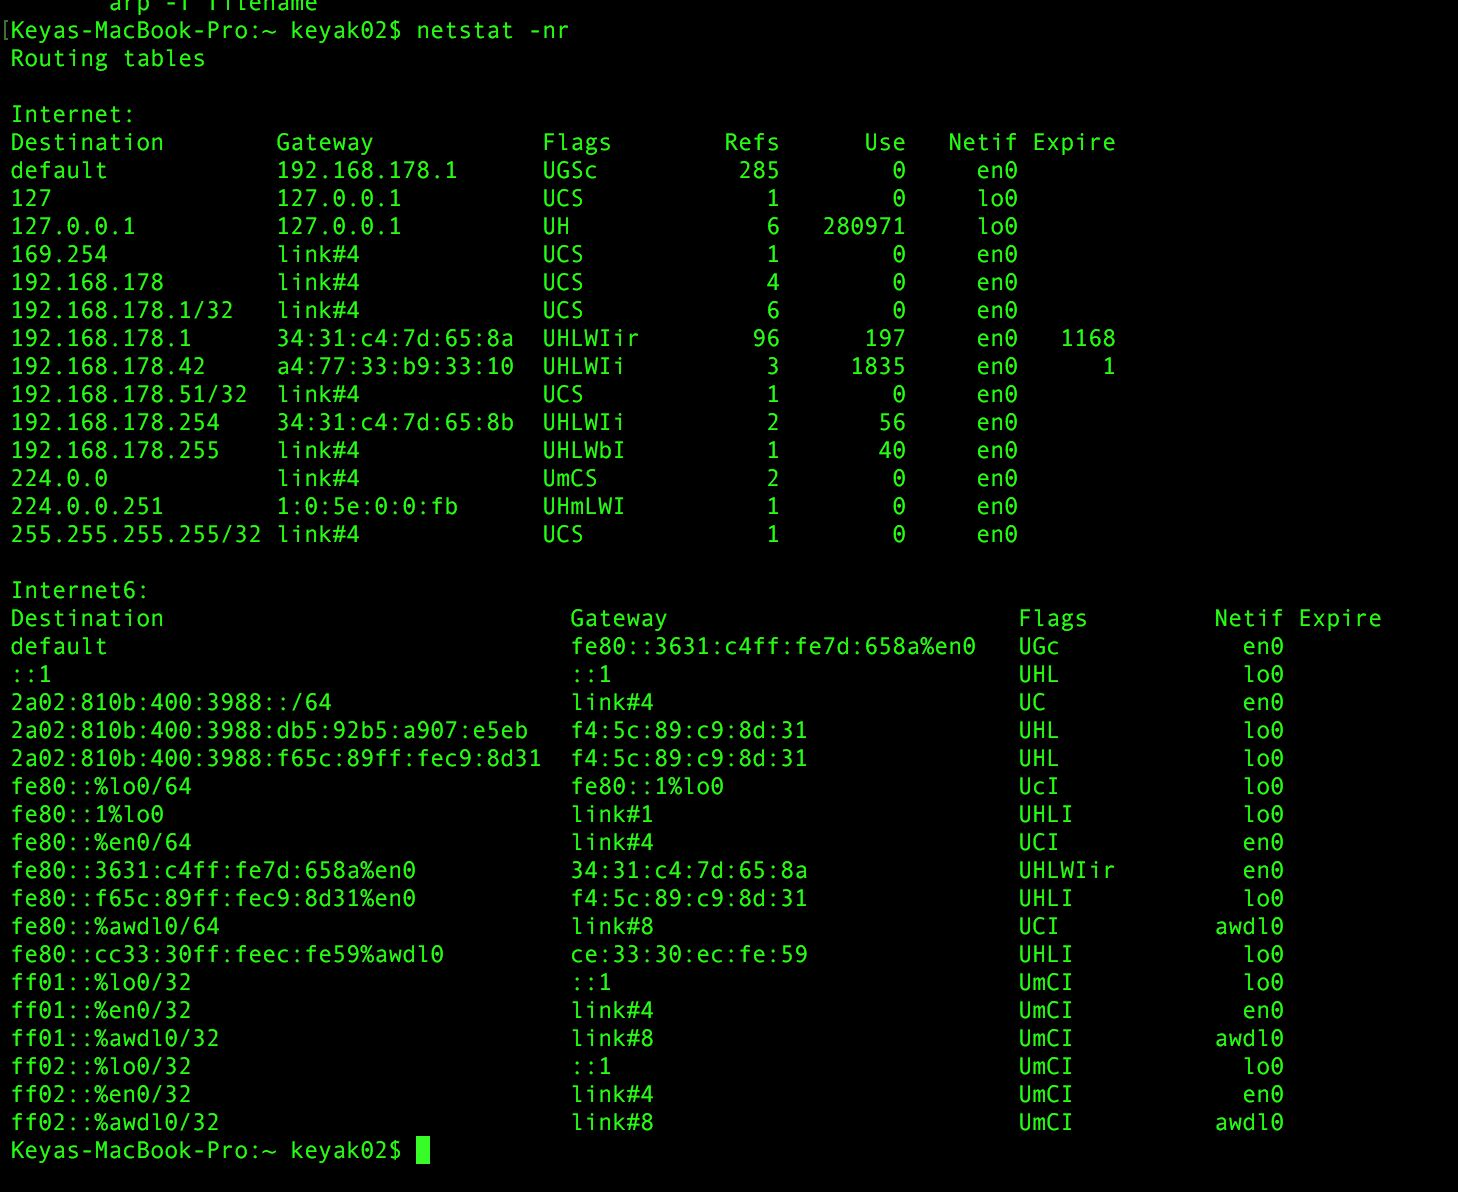
\includegraphics[width=1\textwidth]{images/out-gateway-mac(6-0).png}
\\
\end{enumerate}

% ------------------------------------------------------------------------------

\section{Simple Python Programming (10 Points)}

Write a simple \underline{python program that does the following}:
\begin{enumerate}
\item Generate a random number sequence of 10 values between 0 to 90. 
\item Perform \texttt{sine} and \texttt{cosine} operation on numbers generated. 
\item Store the values in two different arrays named SIN \& COSIN respectively. 
\item Plot the values of SIN \& COSIN in two different colors. 
\item The plot should have labeled axes and legend.
\end{enumerate}

%Answer
\underline{Answers:}
\begin{enumerate}
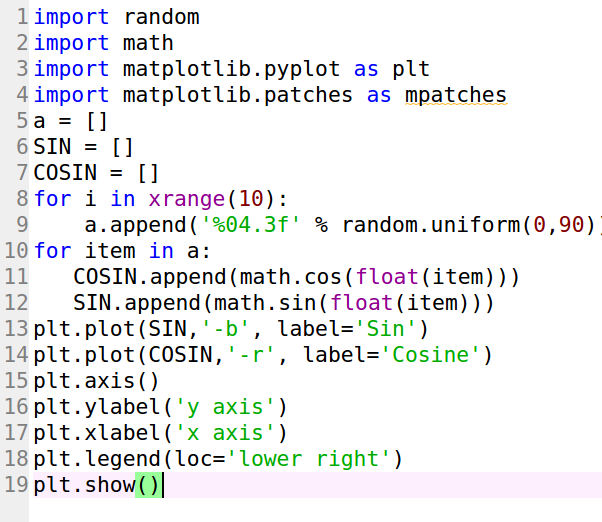
\includegraphics[width=1\textwidth]{images/python-code.png}
\end{enumerate}



\makefooter

\end{document}
